%!TEX root = ../../../report.tex
\section{Assembly} % (fold)
\label{sec:assembly}
Due to the fact that basically all the parts have been linked making use of 3D-printed parts, and all the tolerances of these have been adjusted individually, the assembly has been found easy and fast.
The mounting process has proved to be rapid enough to change some of the parts, as the springs, within minutes.
Furthermore, in the event of mechanical failure of any of the 3D-printed parts, its production and replacement is simple enough to reduce the maintenance time.
This result of employing 3D-printed parts can be considered as one of the main advantages of the whole platform.
The tension of the belts have been adjusted experimentally as explained in the section \ref{sub:pulleys_and_belts} using the zip ties installed.
In Figure \ref{fig:photo_robot_walking}, the complete robot assembled is shown while in \ref{fig:photo_dacbot}, a size comparison between the DACbot \cite{dacbot1} and RuBi can be done.

\begin{figure}[ht!]
    \centering
    \begin{subfigure}[b]{0.39\textwidth}
        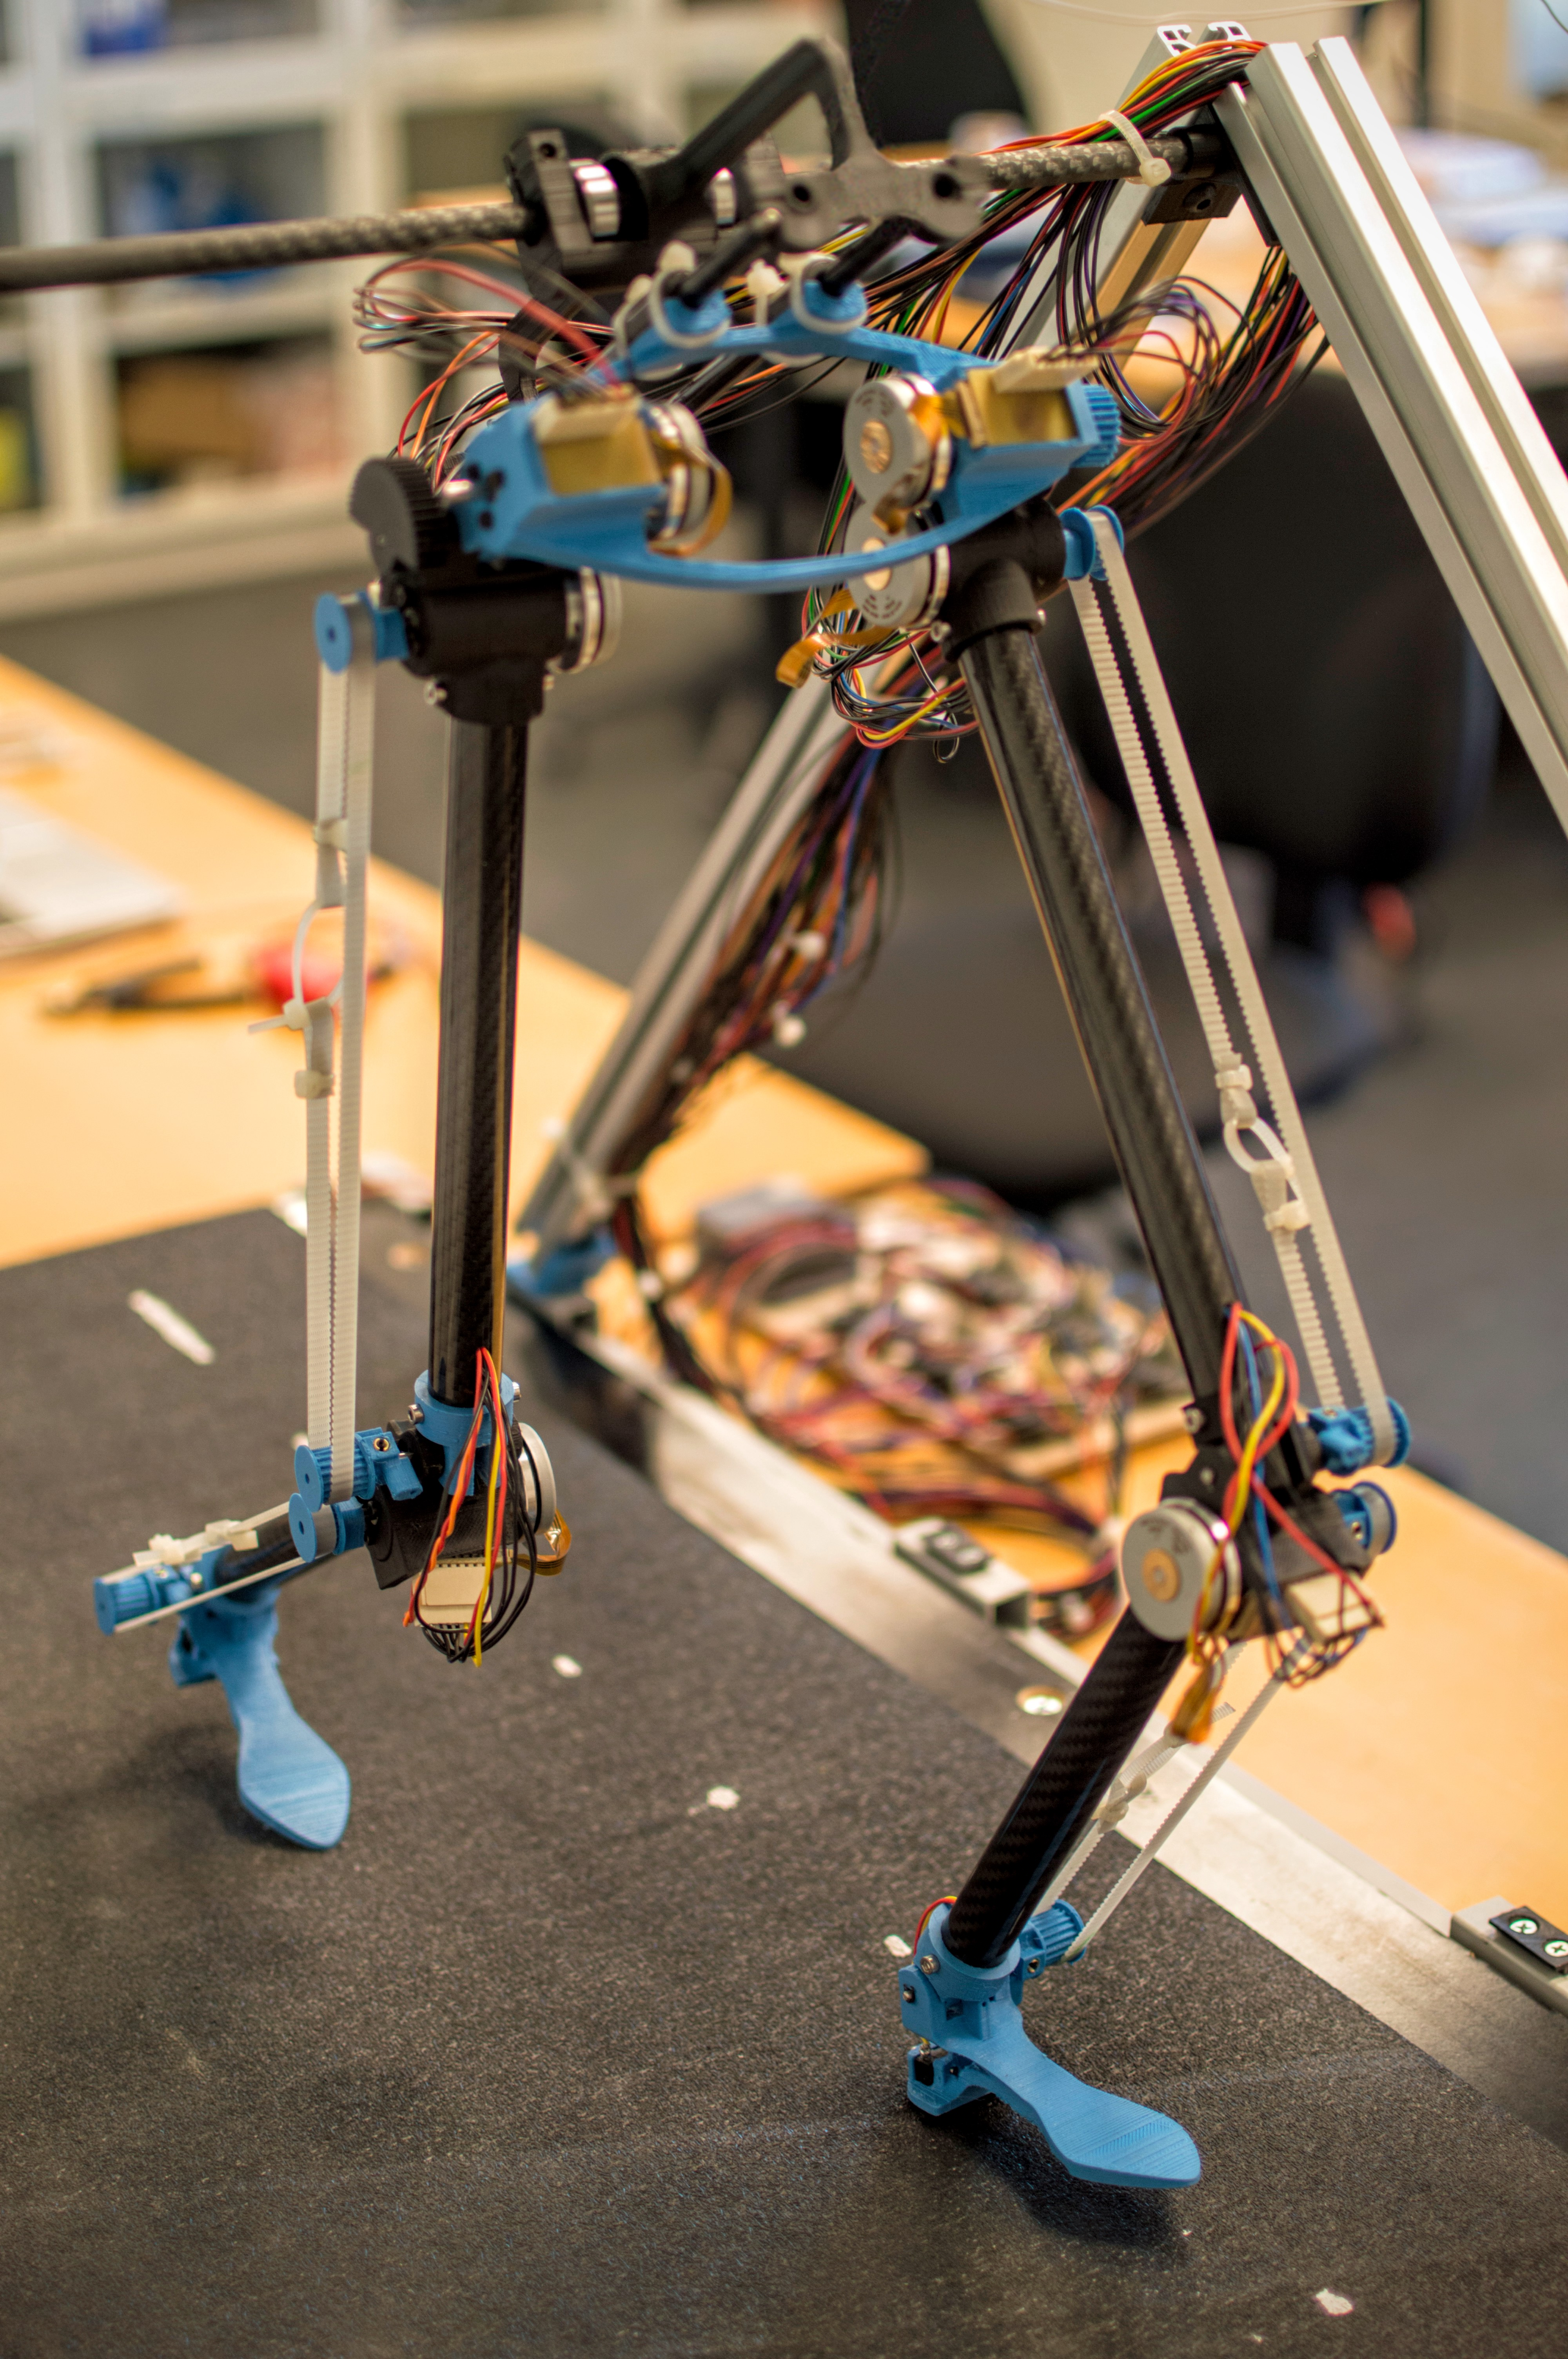
\includegraphics[width=\textwidth]{figures/photo_robot_walking.jpg}
        \caption{RuBi assembled.}
        \label{fig:photo_robot_walking}
    \end{subfigure}
    \begin{subfigure}[b]{0.39\textwidth}
        \includegraphics[width=\textwidth]{figures/photo_dacbot.jpg}
        \caption{RuBi and DACbot.}
        \label{fig:photo_dacbot}
    \end{subfigure}
    \caption{Actual photos of RuBi.}
\end{figure}    
% section assembly (end)